\documentclass[25pt, a0paper, portrait]{tikzposter}
\usepackage[utf8]{inputenc}
\usepackage{graphicx}
\usepackage{epstopdf}
\usepackage{hyperref}
\usepackage{tikz}
\usepackage{amsmath}
\usepackage[mode=build]{standalone}

\tikzposterlatexaffectionproofoff

\graphicspath{ {images/} }

\usetheme{Default}

\definecolor{lightblue}{HTML}{e3f9ff}

\colorlet{blockbodybgcolor}{white}
\colorlet{backgroundcolor}{lightblue}

\settitle{
    \setlength\tabcolsep{0pt}
    \begin{tabular}{lcr}
        \parbox{0.15\linewidth}{
            \centering
            {\LARGE
                \textit{Author}:\\ Ryan Gibb\\
                \textit{Supervisor}:\\ Saleem Bhatti\\
            }
        } &
        \parbox{0.7\linewidth}{
            \centering
            \vspace*{1em}
            {\Huge\scshape CS4099 Demo\\}
            {\LARGE
                Ubiquitous Communication for the Internet of Things\\
                An Identifier-Locator addressing split overlay network\\
            }
            \vspace*{1em}
            {\Large
                School of Computer Science\\
                University of St Andrews\\
            }
        } &
        \parbox{0.15\linewidth}{
            
\includegraphics[scale=10,trim={0.45cm 0.75cm 0.45cm 0.45cm},clip]{st_a_logo.eps}
        } \\
    \end{tabular}
    \setlength\tabcolsep{6pt}
}

\begin{document}

\maketitle

\begin{columns}
    \column{0.33}
    \block{Background}{
        \begin{itemize}
            \item Ubiquitous Computing and the Internet of Things.
            
            \item Mobility in IP.
            
            \begin{itemize}
                \item Overloading of IP address semantics.
                \item Entanglement of layers.
            \end{itemize}
            
            \item Identifier-Locator Network Protocol (ILNP).
            
        \end{itemize}
        \begin{center}
            \begin{tabular}{| l | c | c |} 
                \hline
                Protocol layer & ILNP & IP \\
                \hline\hline
                Application & FQDN & FQDN, IP address \\
                \hline
                Transport & Identifier, \textit{I} & IP address \\
                \hline
                Network & Locator, \textit{L} & IP address \\
                \hline
                (interface) & dynamic binding & IP address \\
                \hline
            \end{tabular}
            ILNP and IP use of names
        \end{center}
    }
    
    \block{An ILNP Overlay Network}{
        \begin{itemize}
            \item Created in userspace with Python.
            \item Focus on protocol design and interaction.
            \item Evaluated with experimental analysis in IoT scenario (Raspberry Pis).
        \end{itemize}
        \includestandalone[width=\linewidth]{diagrams/overlay_network_stack}\\
    }
    
    \column{0.33}
    \block{Discovery Protocol Example}{
        \begin{itemize}
            \item Similar to IPv6 Neighbour Discovery.
            \item Includes hostname resolution.
            \item Packets used for backwards learning.
            \item Bootstarts network by populating forwarding table.
        \end{itemize}
        \includestandalone[width=\linewidth]{diagrams/discovery_protocol_topology}\\
        \includestandalone[width=\linewidth]{diagrams/discovery_protocol_sequence_diagram}\\
    }
    
    \column{0.33}
    \block{Locator Update Protocol Example}{
        \begin{itemize}
            \item ILNP supports seamless connectivity through soft handoffs for layer 3 network transitions.
            \item MN discovery advertisement is for CN to learn where to forward packets to the new locator (\texttt{0:0:0:c}).
            \item Locator update informs all hosts in a unicast communication session with MN of new locator.
        \end{itemize}
        \includestandalone[width=\linewidth]{diagrams/locator_update_topology}\\
        \includestandalone[width=\linewidth]{diagrams/locator_update_sequence_diagram}\\
    }
\end{columns}

\begin{columns}
    \column{0.33}
    \block{Experiment Setup}
    {
        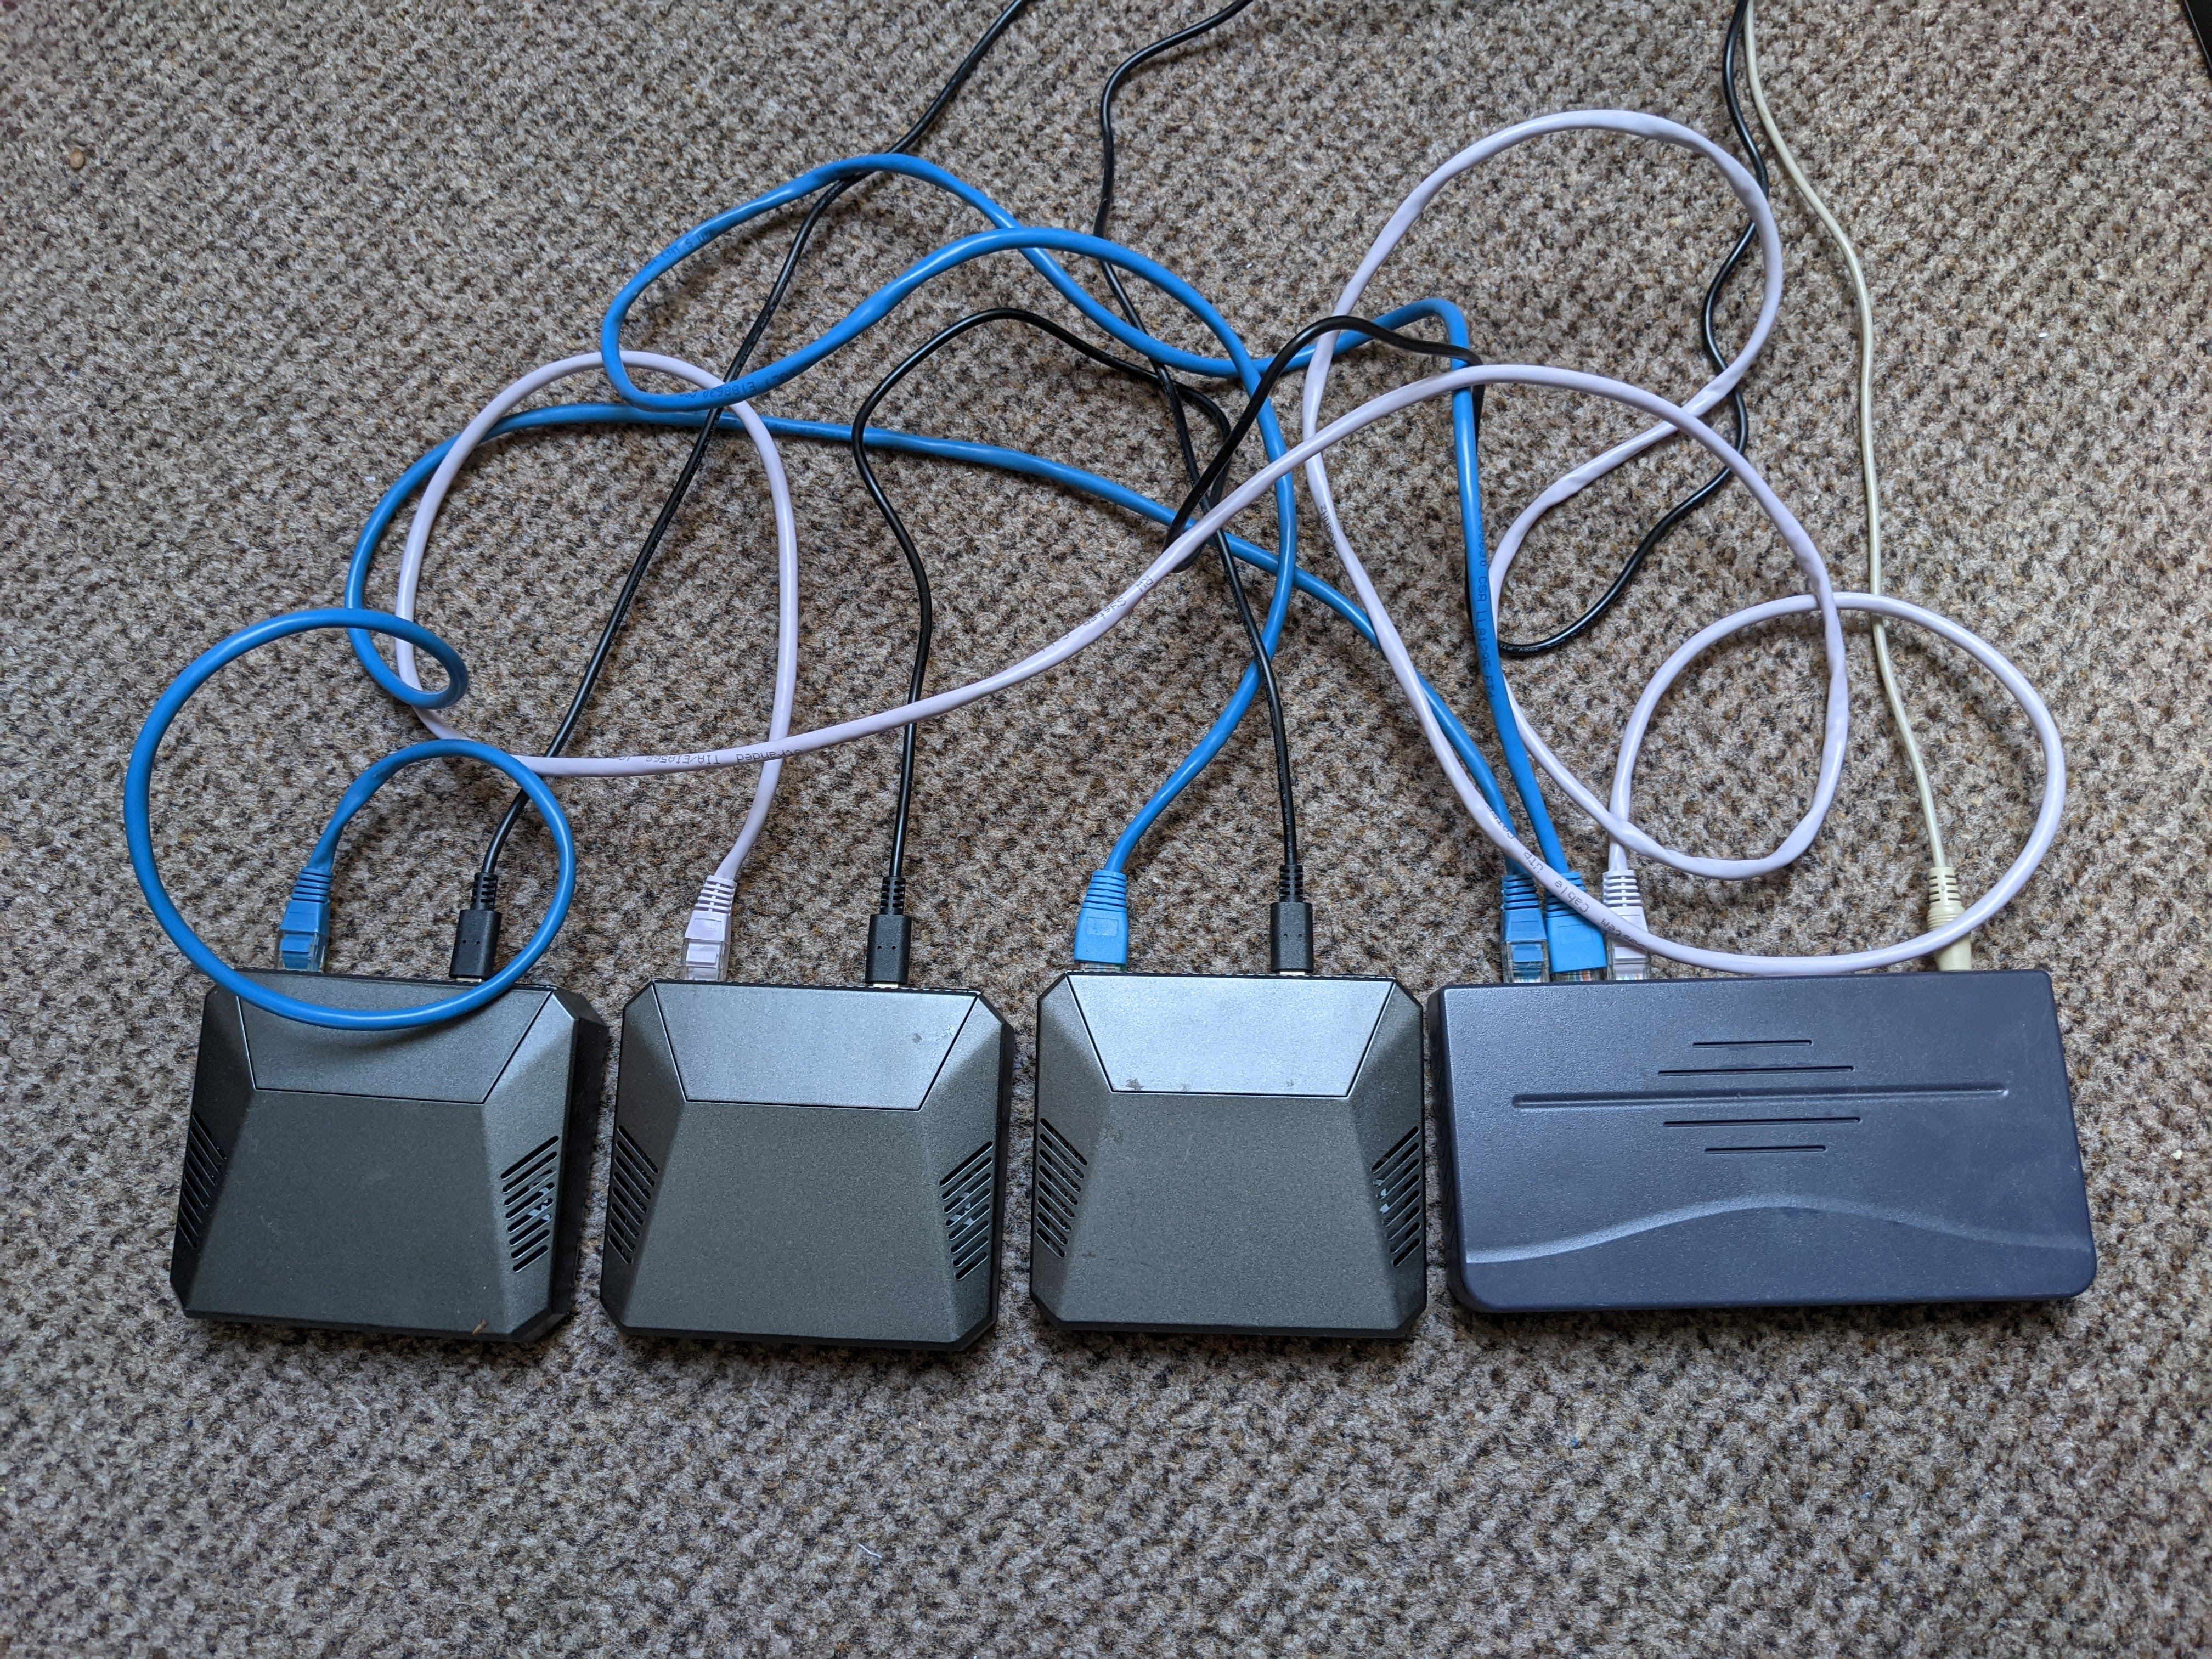
\includegraphics[width=\linewidth]{testbed.jpg}\\
        \includestandalone[width=\linewidth]{diagrams/experiment}\\
    }

    \column{0.33}
    \block{Experiment 3 MN\textless-\textgreater CN}
    {
        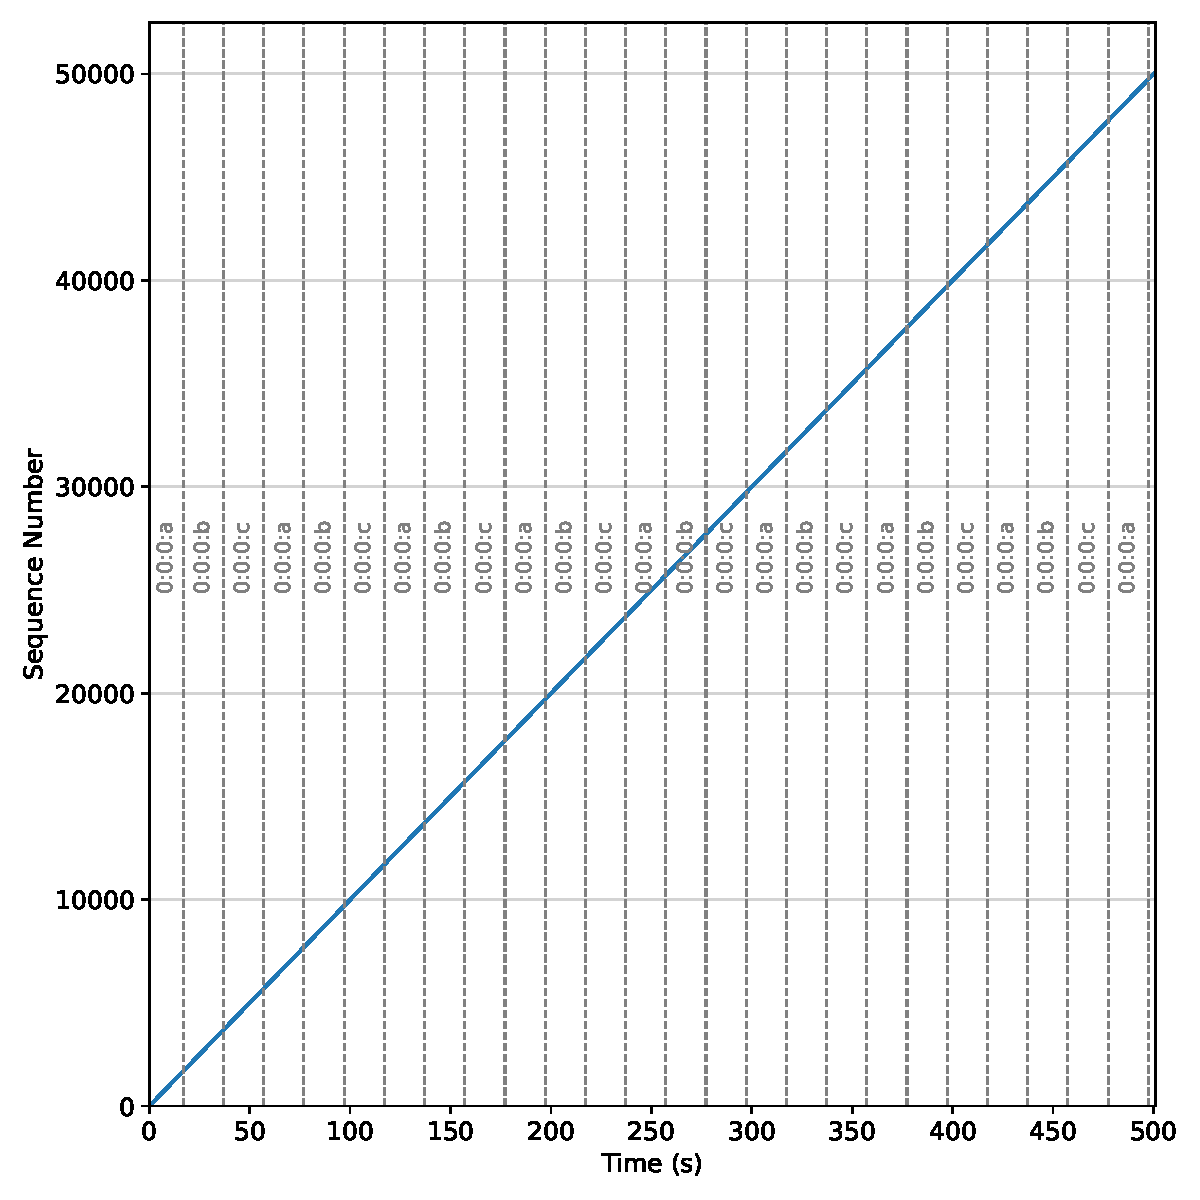
\includegraphics[width=0.5\linewidth]{graphs/exp3/Received sequence numbers vs Time on MN.pdf}
        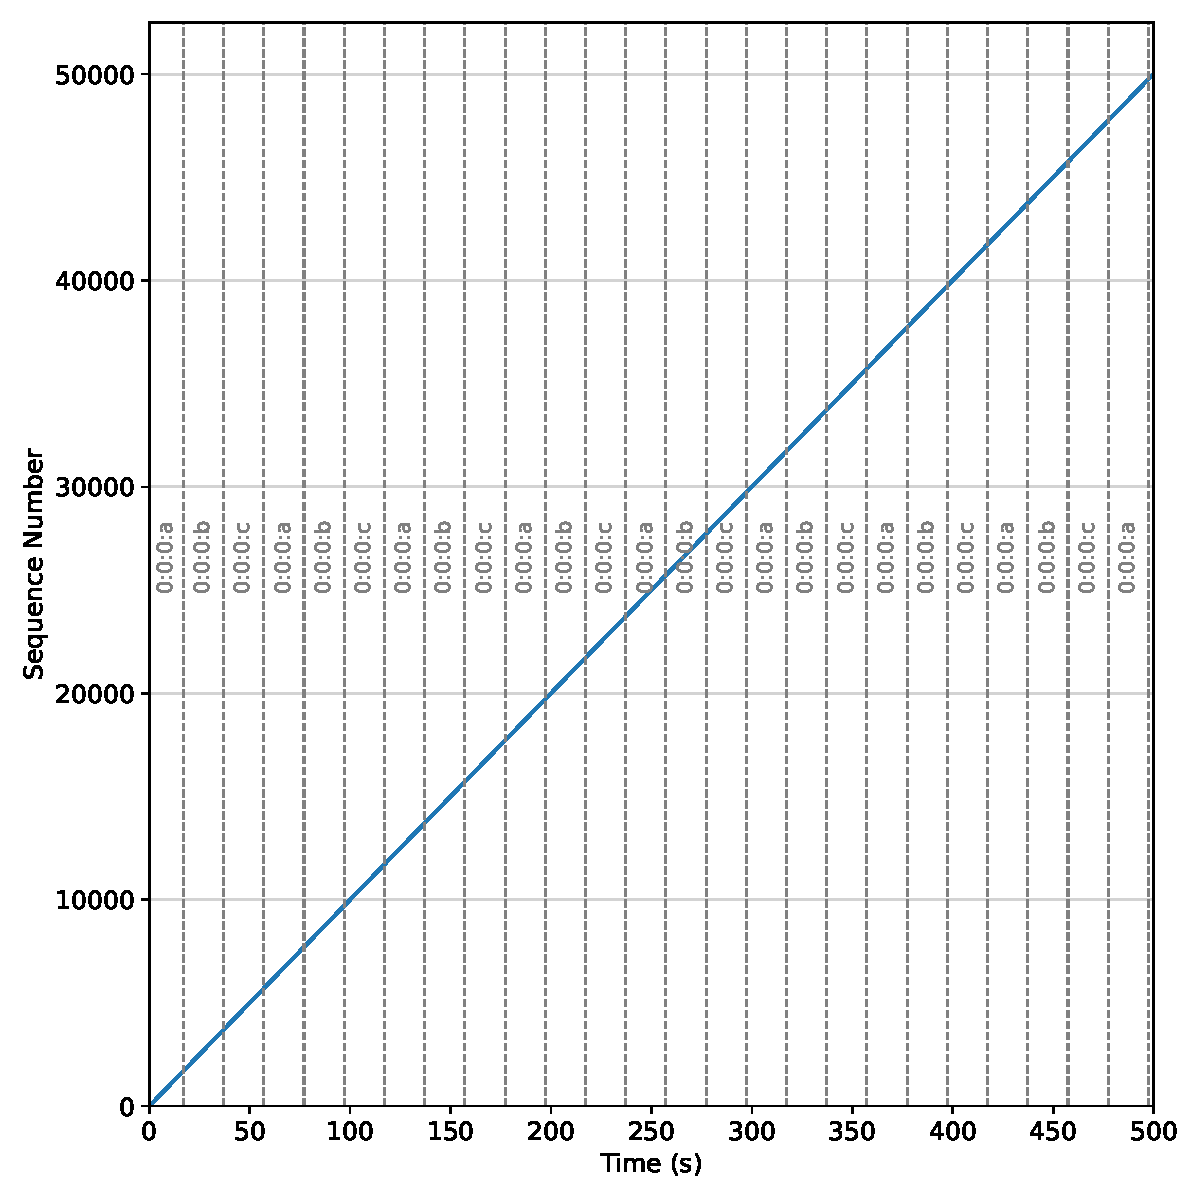
\includegraphics[width=0.5\linewidth]{graphs/exp3/Received sequence numbers vs Time on CN.pdf}
        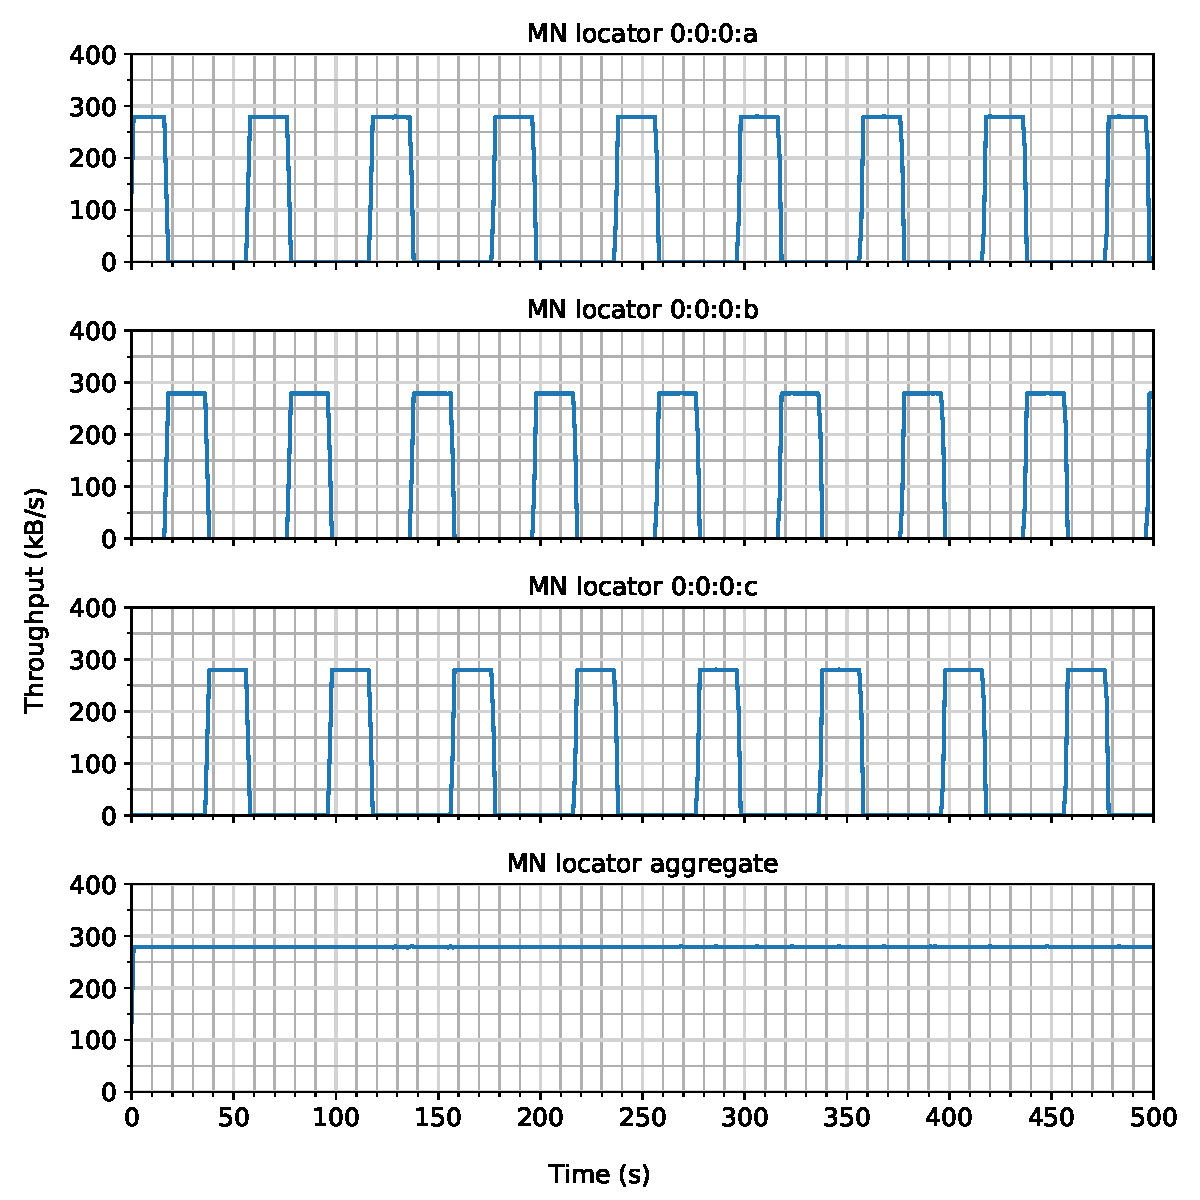
\includegraphics[width=0.5\linewidth]{graphs/exp3/Throughput in 1s buckets vs Time on CN.pdf}
        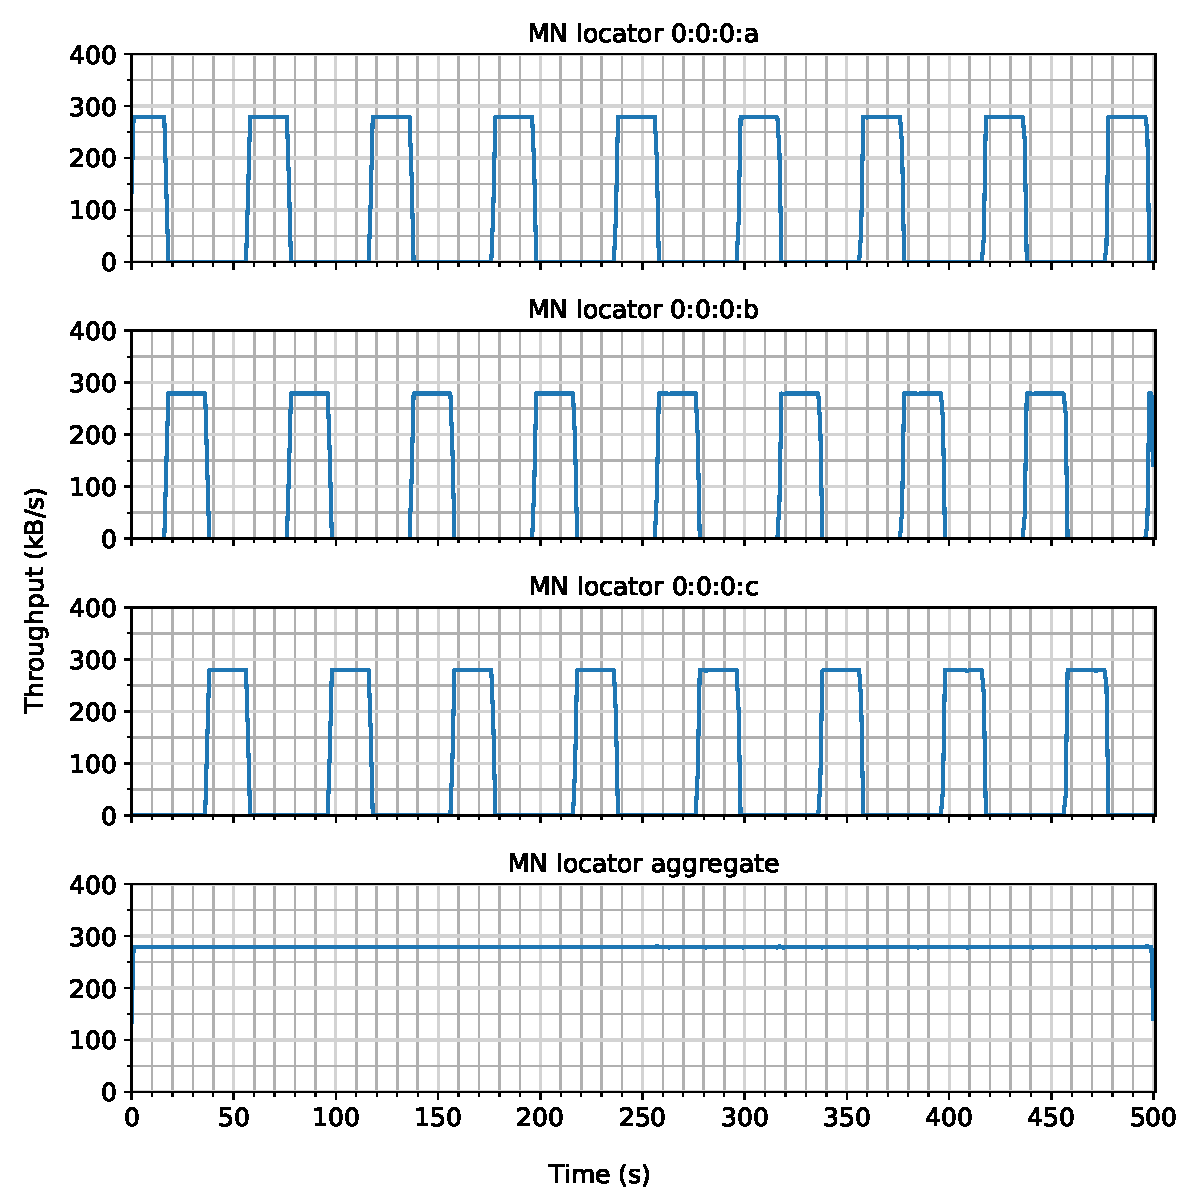
\includegraphics[width=0.5\linewidth]{graphs/exp3/Throughput in 1s buckets vs Time on MN.pdf}
        \begin{itemize}
            \item Bidirectional flow of 1388 byte packets between CN and MN every 10ms.
            \item Smooth receival of sequence numbers across network transitions.
            \item Rectangular throughputs for each locator shows distinct separation between locator uses.
            \item Aggregate throughput shows smooth connectivity across network moves.
        \end{itemize}
    }
    
    \column{0.33}
    \block{Systems Stability Issues}
    {
        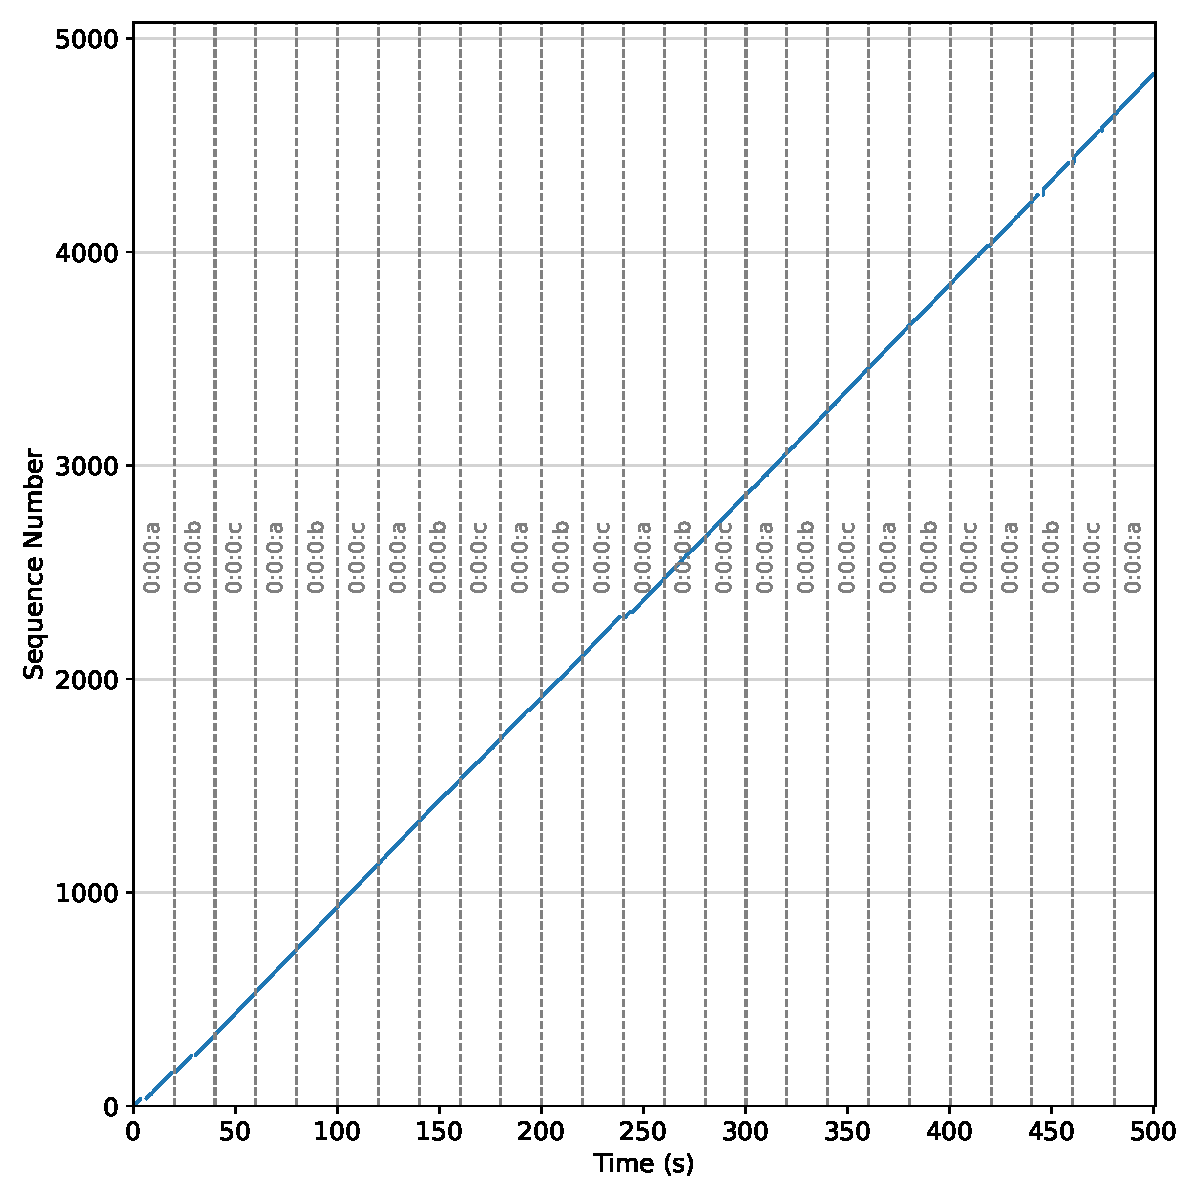
\includegraphics[width=0.5\linewidth]{systems_issues_graphs/exp3/Received sequence numbers vs Time on MN.pdf}
        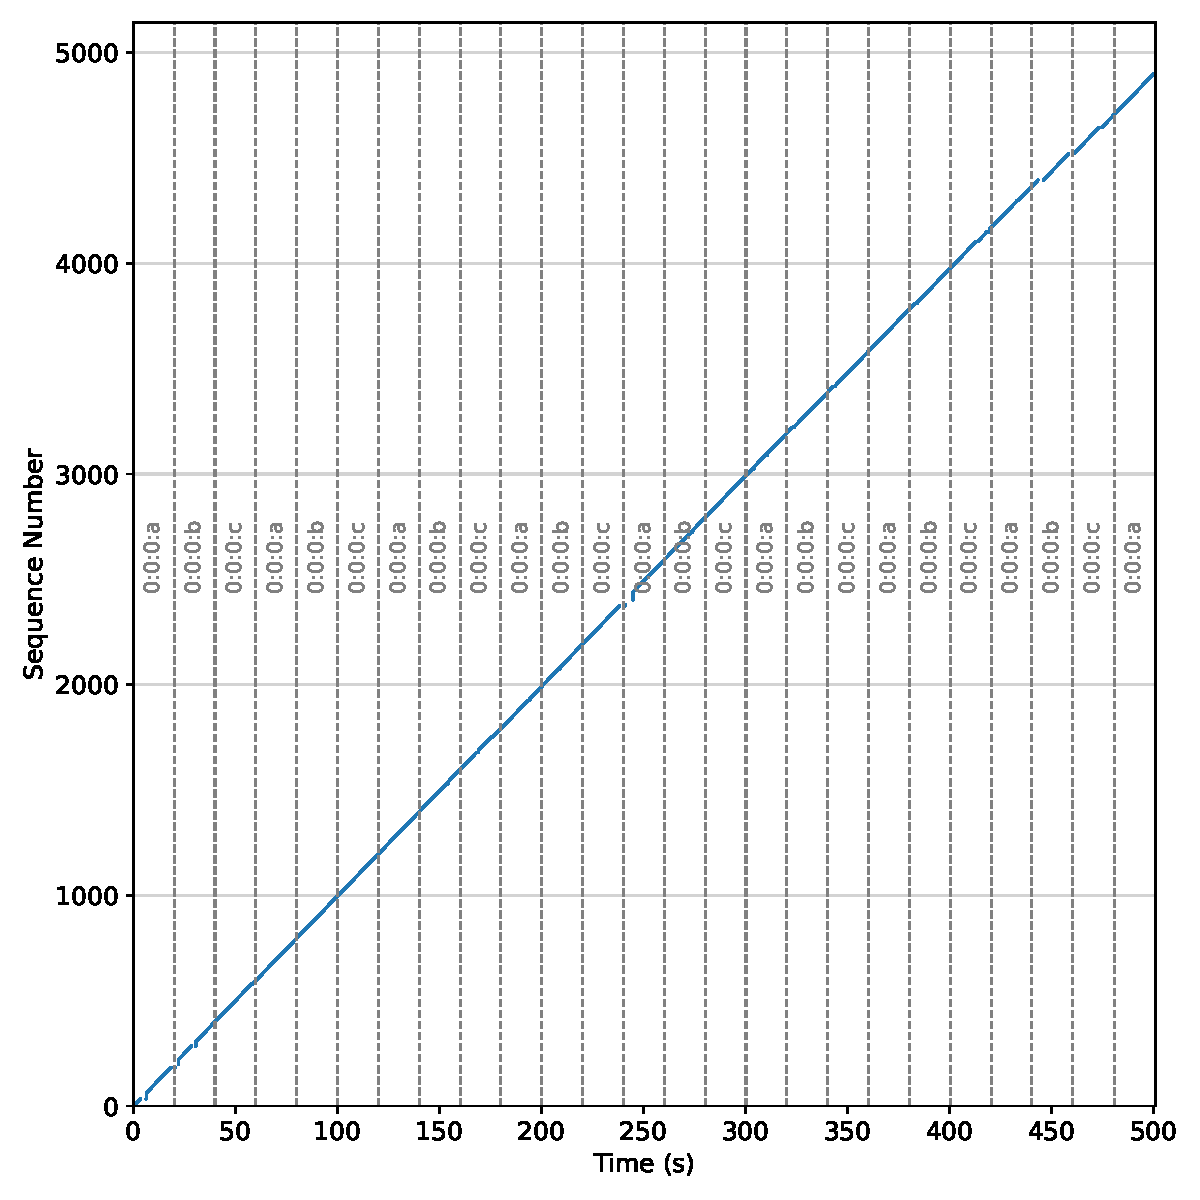
\includegraphics[width=0.5\linewidth]{systems_issues_graphs/exp3/Received sequence numbers vs Time on CN.pdf}
        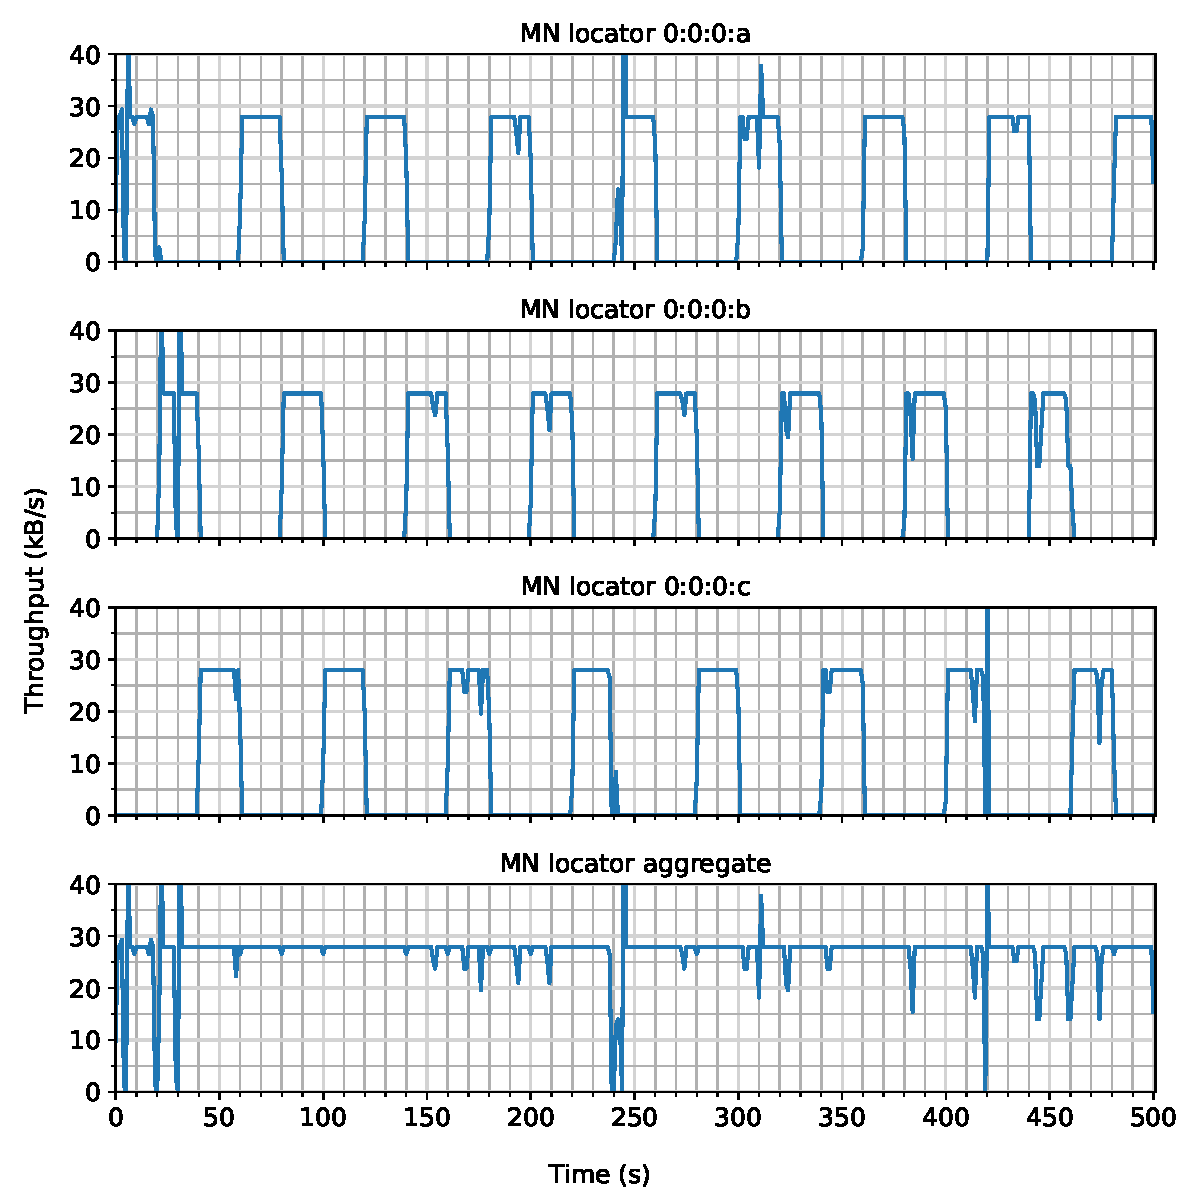
\includegraphics[width=0.5\linewidth]{systems_issues_graphs/exp3/Throughput in 1s buckets vs Time on CN.pdf}
        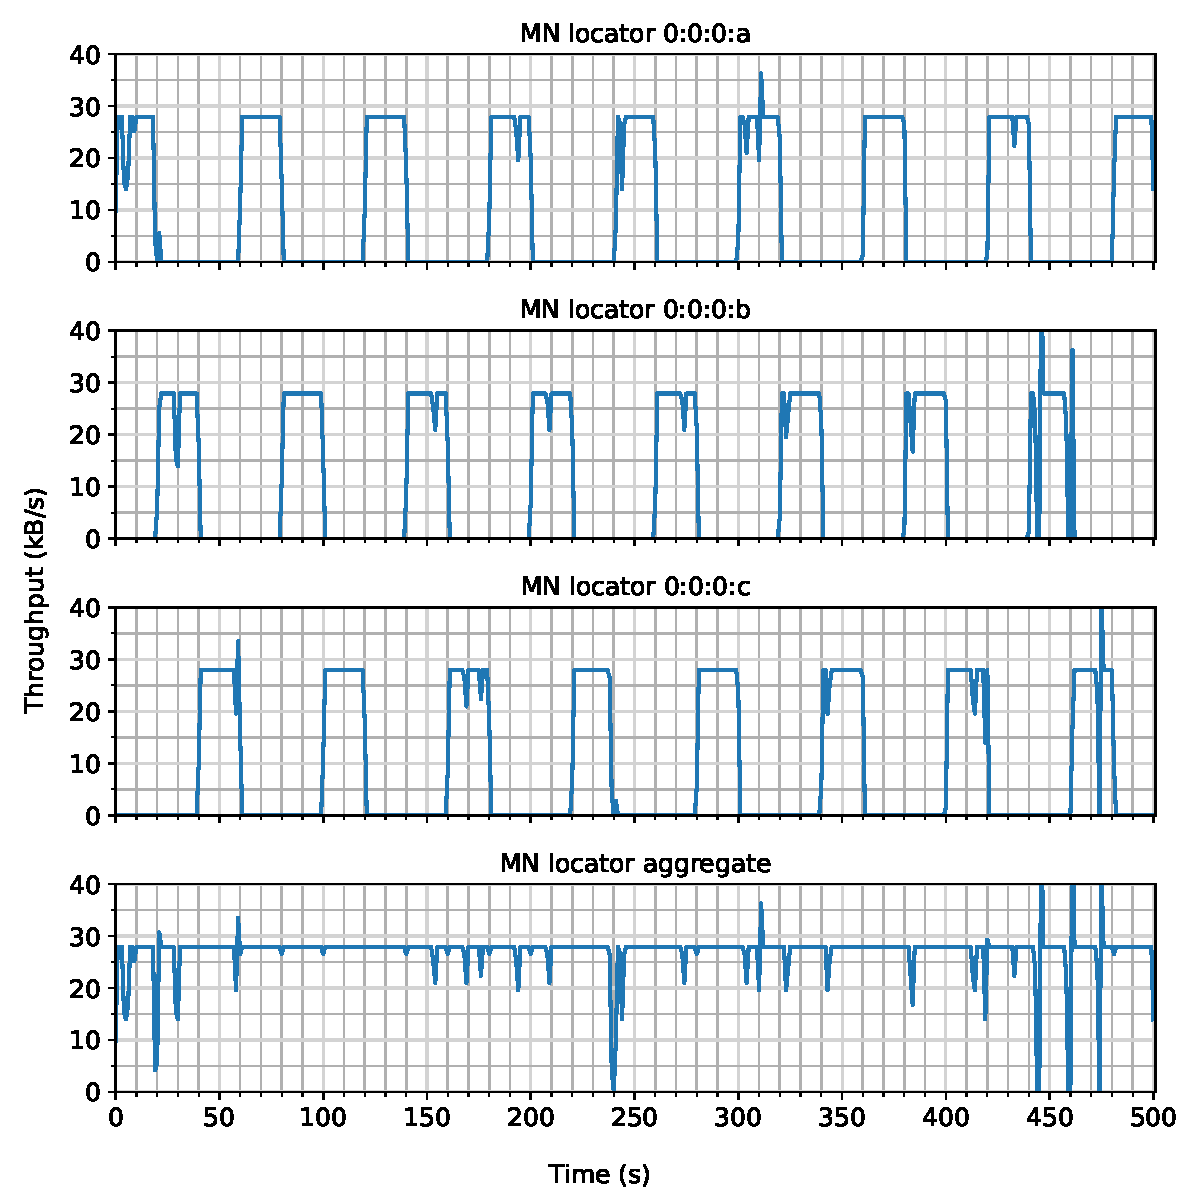
\includegraphics[width=0.5\linewidth]{systems_issues_graphs/exp3/Throughput in 1s buckets vs Time on MN.pdf}
        \begin{itemize}
            \item This is exactly what we \textit{don't} want to see: gaps in sequence numbers, and drops \& spikes in throughput.
            \item This was caused by disk I/O resulting in processes being suspended, due to poor write performance when flushing page cache.
        \end{itemize}
    }
\end{columns}

\end{document}
